% \section{Forms API}
\section{表单 API}

% The exported API of the @Angular/Forms package can be sub-divided into four groups
% – main, directives, accessors and validator directives.

@Angular/Forms 暴露的 API 接口大致可以分为四组:main、directives、accessors 和 validator directives。

% The main group can be represented as:

main 大致可表示为:

% \begin{figure}[!hbt]
%   \centering
%   \caption{@Angular/Forms API (main)}
%   \centerline{
%   \xymatrix {
%   *+[F]\txt{FormsModule} & & *+[F]\txt{ReactiveFormsModule} \\
%   *+[F]\txt{NG\_ASYNC\_VALIDATORS} & & *+[F]\txt{NG\_VALIDATORS} \\
%   *+[F]\txt{Validators} & & *+[F]\txt{FormBuilder} \\
%   & *+[F]\txt{AbstractControl} &  \\
%   *+[F]\txt{FormControl} \ar[ru] & *+[F]\txt{FormGroup} \ar[u] & *+[F]\txt{FormArray} \ar[lu]
%   }
%   }
% \end{figure}

% \begin{figure}[!hbt]
%   \centering
%   \fbox{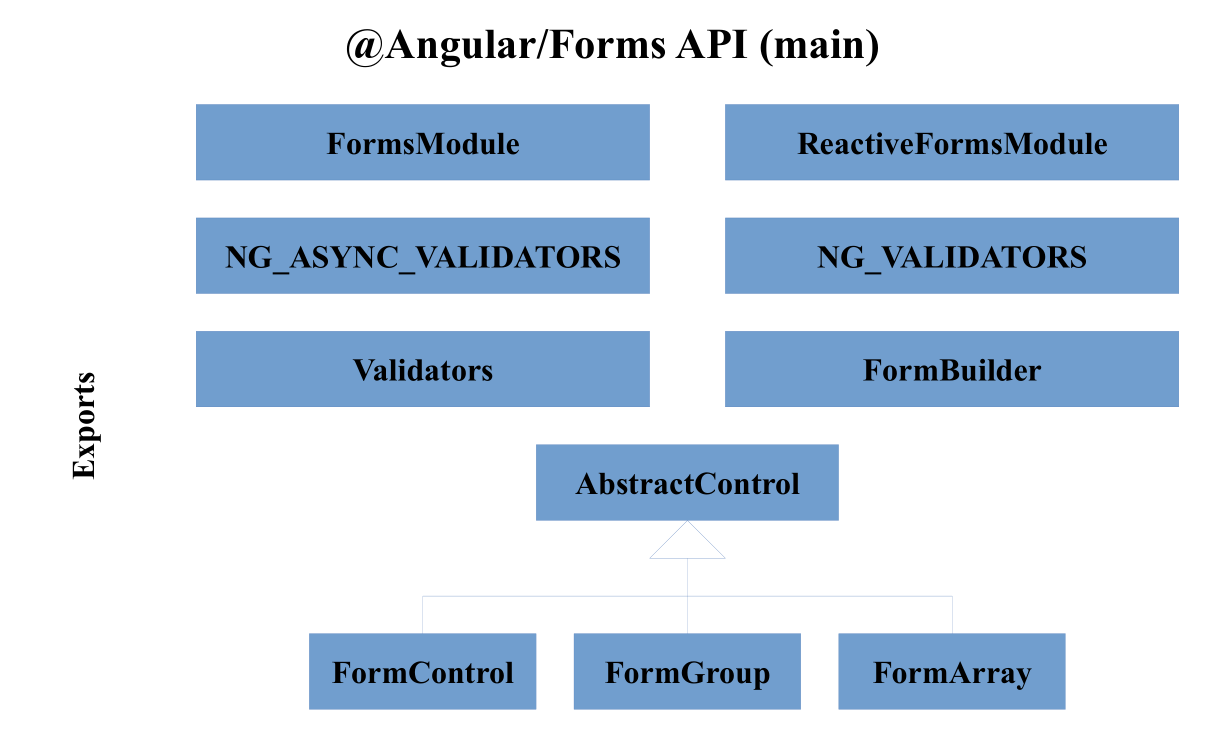
\includegraphics[width=0.9\linewidth]{15_the_forms_package/forms_api}}
%   \label{fig:formsapi}
% \end{figure}

% Its index.ts file contains this one line:

它的 index.ts 文件内容如下:

\begin{minted}{typescript}
export * from './src/forms';
\end{minted}


% The parts of forms.ts related to exporting the above are:

form.ts 中与上述内容相关的导出是:

\begin{minted}{typescript}
export { FormBuilder } from './form_builder';
export { AbstractControl, FormArray, FormControl, FormGroup } from './model';
export { NG_ASYNC_VALIDATORS, NG_VALIDATORS, Validators } from './validators';
export * from './form_providers';
\end{minted}


% Two NgModules are supplied, one for normal forms, FormsModule, and the other for
% reactive forms, ReactiveFormsModule. The control hierarchy starts with a root, and
% has FormControl for actual controls,and two combinations of controls, one for group
% (of fixed size) and one for array (of dynamic size).

还提供了两个 NgModules,一个是 FormsModule,用于普通表单,
另一个是 ReactiveFormsModule,用于响应式表单。
表单控件层次结构从根开始,FormControl 用于实际的控件,
以及两种控件组合,一种是表单组(固定大小),
另一种用于数组(动态大小)

% A large directive hierarchy is supplied for both types of forms:

为两种类型的表单提供了一个大的指令继承结构:

% \begin{figure}[!hbt]
%   \centering
%   \fbox{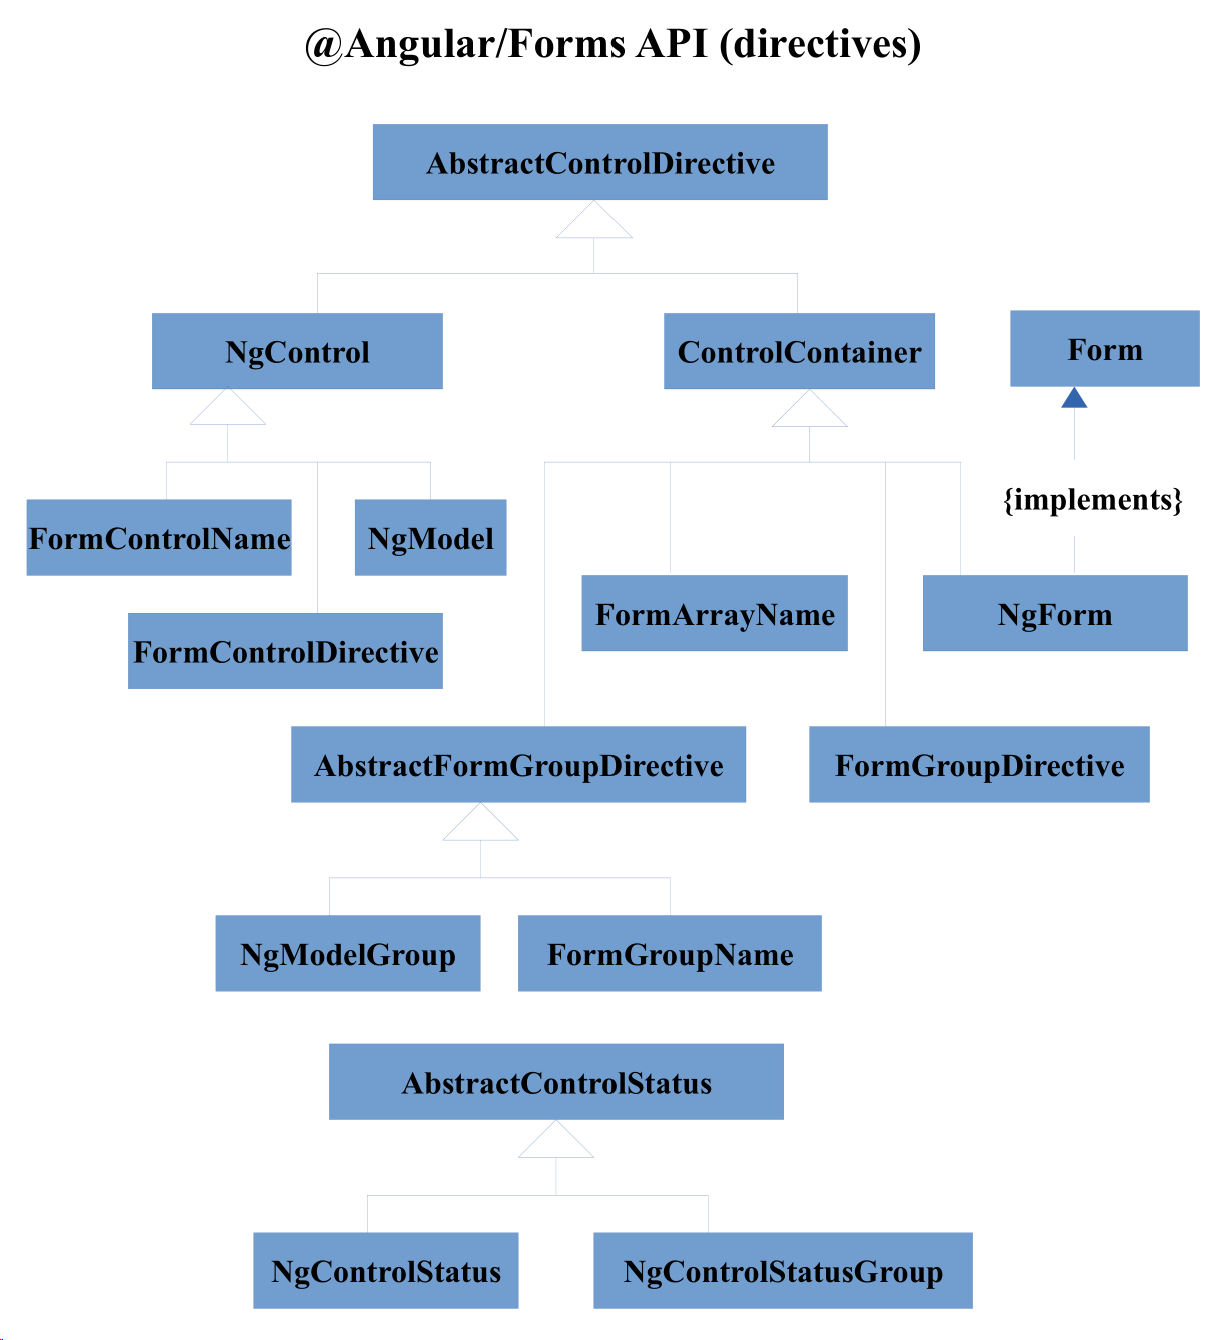
\includegraphics[width=0.9\linewidth]{15_the_forms_package/forms_api_directive}}
%   \label{fig:formsapidirective}
% \end{figure}

% The parts of forms.ts related to exporting directives are:

forms.ts 中与指令导出相关的部分是:

\begin{minted}{typescript}
export { AbstractControlDirective } from './directives/abstract_control_directive';
export { AbstractFormGroupDirective } from './directives/abstract_form_group_directive';
export { ControlContainer } from './directives/control_container';
export { Form } from './directives/form_interface';
export { NgControl } from './directives/ng_control';
export {
  NgControlStatus,
  NgControlStatusGroup,
} from './directives/ng_control_status';
export { NgForm } from './directives/ng_form';
export { NgModel } from './directives/ng_model';
export { NgModelGroup } from './directives/ng_model_group';
export { FormControlDirective } from './directives/reactive_directives/form_control_directive';
export { FormControlName } from './directives/reactive_directives/form_control_name';
export { FormGroupDirective } from './directives/reactive_directives/form_group_directive';
export { FormArrayName } from './directives/reactive_directives/form_group_name';
export { FormGroupName } from './directives/reactive_directives/form_group_name';
\end{minted}


% The accessor hierarchy can be represented as:

访问器层次结构可以表示为:

% \begin{figure}[!hbt]
%   \centering
%   \fbox{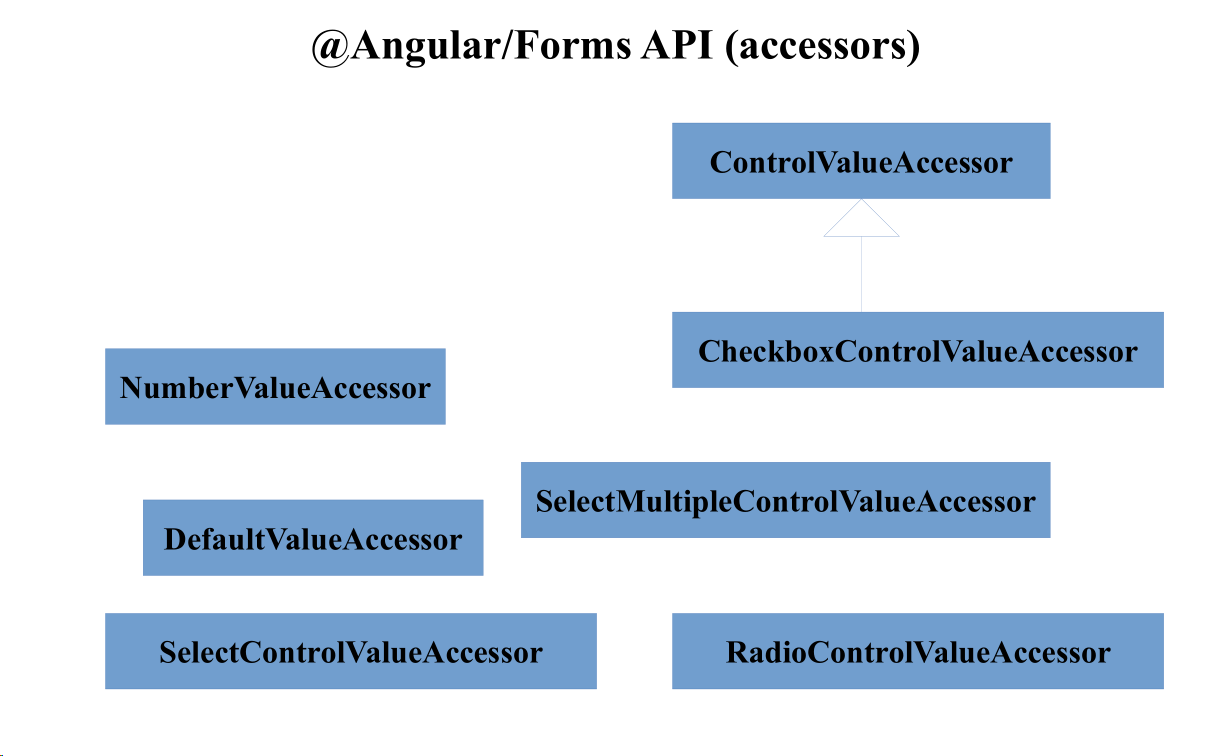
\includegraphics[width=0.9\linewidth]{15_the_forms_package/form_api_accessors}}
%   \label{fig:formapiaccessors}
% \end{figure}

% The parts of forms.ts related to exporting accessors are:

form.ts 中与访问器相关的部分是:

\begin{minted}{typescript}
export { CheckboxControlValueAccessor } from './directives/checkbox_value_accessor';
export {
  ControlValueAccessor,
  NG_VALUE_ACCESSOR,
} from './directives/control_value_accessor';
export { DefaultValueAccessor } from './directives/default_value_accessor';
export {
  NgSelectOption,
  SelectControlValueAccessor,
} from './directives/select_control_value_accessor';
export { SelectMultipleControlValueAccessor } from './directives/select_multiple_control_value_accessor';
\end{minted}


% The part of forms.ts related to exporting validator directives is:

和验证指令相关的部分是:

% \begin{figure}[!hbt]
%   \centering
%   \fbox{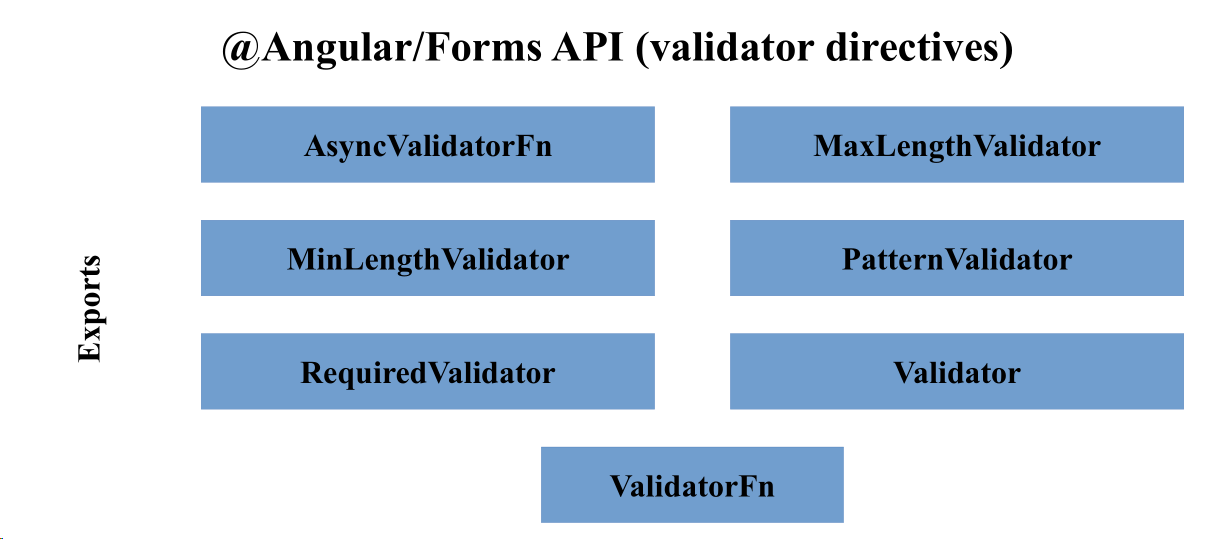
\includegraphics[width=0.9\linewidth]{15_the_forms_package/forms_api_validator}}
%   \label{fig:formsapivalidator}
% \end{figure}

\begin{minted}{typescript}
export {
  AsyncValidatorFn,
  MaxLengthValidator,
  MinLengthValidator,
  PatternValidator,
  RequiredValidator,
  Validator,
  ValidatorFn,
} from './directives/validators';
\end{minted}

